%!TEX root = "../../../DA_GUI.tex"

%	--------------------------------------------------------
% 	Debugger: Einleitung
%	--------------------------------------------------------

\section{Einleitung}

%   --------------------------------------------------------
%   Grundlegende Funktionen, Ideen
%   --------------------------------------------------------

\subsection{Die grundlegende Idee}
Ein wichtiger Bestandteil von C Compact ist der integrierte eigene Debugger, der speziell für die Bedürfnisse von Anfängern ausgelegt ist. Während das Programm Schritt für Schritt abgearbeitet wird, sind alle Variablen und der Call Stack in übersichtlicher Form dargestellt. In der Variablentabelle werden Wertänderungen farbig hervorgehoben. Dadurch soll ein fundiertes Verständnis für den Programmablauf und die Logik dahinter entstehen.

Ein daraus resultierender Vorteil ist, dass Schüler von Anfang an mit einem Debugger arbeiten und ähnliche Tools später auch in anderen Entwicklungsumgebungen verwenden werden.

Da wir Compiler und Interpreter selbst entwickeln, kann die Grafische Oberfläche in den Programmablauf eingreifen und aktuelle Daten abfragen. Des Weiteren haben wir Schutzfunktionen implementiert, die Probleme wie etwa Pufferüberläufe erkennen. Solche Fehler werden besonders von Anfängern leicht übersehen und führen meist zu einem undefinierbaren Verhalten des Programmes.

Fehler im Präprozessor, Compiler oder Interpreter werden dem Benutzer übersichtlich angezeigt und verständlich erklärt. Außerdem werden Hinweise zur Fehlersuche und -behebung gegeben.
%TODO ref: nicht verwechseln mit internen Fehlern

%   --------------------------------------------------------
%   Bedienung des Debuggers
%   --------------------------------------------------------

\subsection{Bedineung des Debuggers}
Bevor die konkrete Implementierung des Debuggers beschrieben wird, soll auf seine grundlegende Bedienung und die Kommunikation mit dem Benutzer eingegangen werden.

\begin{figure}[htp]
\centering
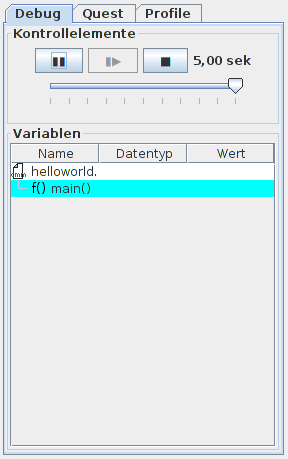
\includegraphics[width=0.4\textwidth]{./media/images/gui/debugger/CCompact-guimain-run.png}
\caption{Bedienungspanel des Debuggers}
\label{fig:deb-gui-rpanel}
\end{figure}

Abbildung \ref{fig:deb-gui-rpanel} zeigt die Bedienelemente des Debuggers, die als Teil des rechten Panels (Siehe Kapitel \ref{sec:gui-main-right-reg-deb}) im Haupfenster von C Compact angezeigt werden. Im oberen Teil befindet sich ein Panel mit Kontrollelementen, darunter werden - wenn der Debugger läuft - Call Stack und Variablen des Programmes angezeigt.

Der Debugger hat vier unterschiedliche Modi, diese wurden bereits in Kapitel \ref{sec:gui-main-left-zust} überblicksmäßig beschrieben. Der Wechsel zwischen diesen zuständen erfolgt durch Eingaben des Benutzers, entweder mit den Kontrollelementen (Buttons) in der Benutzeroberfläche, oder mit Keyboard Shortcuts.
%TODO ref keyboard shortcuts

Mit dem Regler unter den Buttons kann der Zeitabstand eingestellt werden, nach beim automatischen Debuggen zum nächsten Schritt gesprungen wird. Die gewählte Zeit wird, je nach zur Verfügung stehendem Platz, neben oder über dem Regler angezeigt.
%TODO diesen Absatz nochmal lesen

Die vier Zustände sind:
\begin{enumerate}
\item \textbf{Text bearbeiten (ready mode)}
\item \textbf{Fehler aufgetreten (error mode)}
\item \textbf{Programm Schritt für Schritt abarbeiten oder Pause (pause mode)}
\item \textbf{Programm automatisch abarbeiten (run mode)}
\end{enumerate}
%TODO bedienelemente können ausgeblendet werden

Obwohl der Debugger selbst zwischen Modus 1 und 2 unterscheidet, gibt es in der Benutzeroberfläche nur mehr den Editormodus. Der Fehlermodus wird trotzdem im Zustandspanel des Debuggers im Hauptfenster angezeigt, damit der Benutzer auf den aufgetretenen Fehler aufmerksam gemacht wird. Wie in Abbildung \ref{fig:deb-zust-simple} ersichtlich ist, erfüllen die beiden Modi die selben Funktionen.

\begin{figure}[htp]
\centering
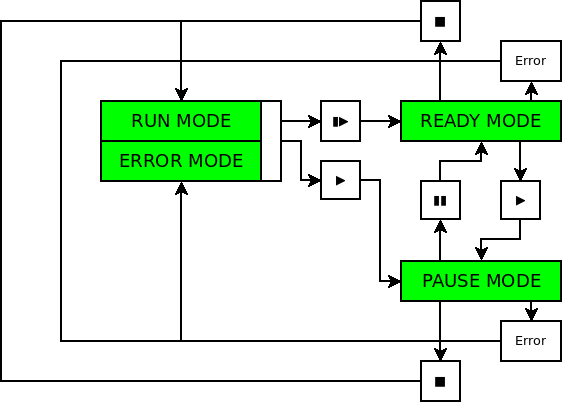
\includegraphics[width=0.65\textwidth]{/home/fabian/Dokumente/C--/CMM/doc/de/media/images/gui/debugger/RunModes_Simple.png}
\caption{Vereinfahctes Zustandsdiagramm des Debuggers}
\label{fig:deb-zust-simple}
\end{figure}

Der dritte Zustand hat zwei Funktionen: einerseits entspricht dieser Modus einer Pausierung (bezogen auf Zustand 4, in dem der Debugger automatisch durchläuft) und andererseits kann in diesem Modus mit dem mittleren Button auch direkt zum nächsten Schritt gesprungen werden.

Ein Sonderfall der 4. Modus ist der ,,quick run mode''. Wenn der Regler für die Zeitabstände zwischen den Schritten des Debuggers auf null gestellt wird, werden die folgenden Schritte so schnell wie möglich abgearbeitet, bis entweder das Programm zu Ende ist oder der Debugger auf einen ,,wait''-Befehl stößt (Siehe Kapitel \ref{})
%TODO ref commands

%   --------------------------------------------------------
%   Schlüsselwörter
%   --------------------------------------------------------

\subsection{Schlüsselwörter}
%TODO ref compiler
%TODO ref panelRunListener
In der Sprache von C Compact gibt es zwei Schlüsselwörter, die zumindest im Endeffekt nicht vom Compiler oder Interpreter, sondern vom Debugger verarbeitet werden.

\subsubsection*{wait}
%TODO ref AST
Dieser Befehl kann an jeder beliebigen Stelle im Programm stehen. Der Compiler baut diesen Befehl als Element im Abstrakten Syntaxbaum ein. Wenn der Debugger diesen Knoten erhält, geht er in den Pause-Modus (3).

\subsubsection*{library}
Das Attribut \textbf{library} kann sowohl an einer Variable, als auch an einer Funktion angewandt werden. Das Schlüsselwort muss immer zwischen Typ und Name der Variable bzw. Funktion stehen.

Eine Variable mit dem \textbf{library}-Attribut wird im Debugger nicht angezeigt. Dies wird zum Beispiel verwendet, um die zahlreichen Konstanten der Bibliothek \textbf{math.h} im Debugger auszublenden.

Hat eine Funktion das \textbf{library}-Attribut, springt der Debugger nicht in diese Funktion, sondern arbeitet sie in einem Schritt ab. Dadurch können Bibliotheksfunktionen im Debugger wie einfache Befehle verwendet werden.
